% Modelo de slides para projetos de disciplinas do Abel
\documentclass[12pt]{beamer}

% \usepackage[utf8]{inputenc}		% Codificação do documento (conversão automática dos acentos)
\usepackage{fontspec}
\usepackage{indentfirst}		% Indenta o primeiro parágrafo de cada seção.
\usepackage{color}				% Controle das cores
\usepackage{graphicx}			% Inclusão de gráficos
\usepackage{microtype} 			% Para melhorias de justificação


\usetheme[progressbar=frametitle, numbering=none]{metropolis}
\usepackage{appendixnumberbeamer}
% \usepackage[numbers,sort&compress]{natbib}
\bibliographystyle{plainnat}

\usepackage{booktabs}
\usepackage[scale=2]{ccicons}

\usepackage{xspace}
\newcommand{\themename}{\textbf{\textsc{metropolis}}\xspace}
% \setbeamertemplate{page number in head/foot}{}

% \setsansfont[BoldFont={Fira Sans SemiBold}]{Fira Sans Book}
\usepackage{cabin}
\usepackage{enumitem}

\pdfstringdefDisableCommands{%
  \def\\{}%
  \def\newline{}%
}

\title{Análise de problemas altamente importantes capazes de serem resolvidos através da computação}

% \subtitle{Aula 2: Tipos de cpp e Análise Exploratória de Berilhes}
% \date{}
\author{Atílio Antônio Dadalto\\Philipe Aguiar Marques\\Tiago da Cruz Santos}
\date{2019}
\institute{UFES}
% \titlegraphic{\hfill\includegraphics[height=1.5cm]{logo.pdf}}

\begin{document}

\maketitle

\section{Problema 1:\newline Gestão de finanças pessoais}

\begin{frame}{O que é o problema}
    \begin{columns}
        \begin{column}{0.65\textwidth}
            \begin{enumerate}[label=•]
                \item Monitorar gastos é complicado e cansativo
        	    \item Dados ficam espalhados em diversos extratos de contas bancárias
        	    \item Adicionar dados manualmente é desestimulante e o usuário pode esquecer
        	    \item Utilizar planilhas pode ser pouco intuitivo
            \end{enumerate}
            \vspace{2mm}
            \textbf{Todos esses fatores requerem muita disciplina do usuário}
        \end{column}
        \begin{column}{0.35\textwidth}
            \begin{center}
                
\includegraphics[width=0.9\textwidth]{figuras/haroldtriste.jpg}
             \end{center}
        \end{column}
    \end{columns}
\end{frame}

\begin{frame}{O que é a solução}
    \begin{columns}
        \begin{column}{0.65\textwidth}
        \textbf{Gestão de finanças integrada a contas bancárias}
        
            \begin{enumerate}[label=•]
                \item Integração com extrato bancário remove um grande obstáculo
    	        \item Centralizar as informações em um único lugar ajuda a ter um panorama geral da situação financeira
    	        \item Relatórios gerados pelo sistema concebem uma nova visão acerca dos gastos
            \end{enumerate}
        \end{column}
        \begin{column}{0.35\textwidth}
            \begin{center}
                
\includegraphics[width=0.9\textwidth]{figuras/haroldsfelizes.jpg}
             \end{center}
        \end{column}
    \end{columns}
\end{frame}

\begin{frame}{Funções principais}
    \begin{enumerate}[label=•]
        \item Acesso distante à cada banco
        \item Monitoramento de extrato bancário com atribuição automática de categorias
        \item Possibilidade de adicionar gastos manualmente
        \item Relatórios e resumos de gastos
        \item Previsão de gastos futuros baseado em parcelamentos feitos e por estimativa com base em dados passados
        \item Informações sobre educação financeira para auxiliar o usuário 
        \item Sistema de sugestões com base em dados anonimizados de outros usuários
    \end{enumerate}
\end{frame}

\begin{frame}{Funções principais}
    \begin{enumerate}[label=•]
        \item Configurar uma renda para previsão de entrada de dinheiro
        \item Configurar limite de gastos para eventual aviso se gastos ultrapassarem o limite
        \item Exportar dados para diversos formatos, como CSV, XML, PDF, etc, bem como importação por CSV
        \item Salvar dados tanto em conta na nuvem como em arquivo no dispositivo
        \item Criação de objetivos (economizar x reais, comprar objeto y)
    \end{enumerate}
\end{frame}

\begin{frame}{Pontos fracos da solução}
    \begin{columns}
        \begin{column}{0.65\textwidth}
            \begin{enumerate}[label=•]
                \item Nem todos os bancos possibilitam/facilitam a conexão
                \item Gastos com dinheiro vivo por exemplo ainda devem ser contabilizados manualmente
                \item Atribuição automática de categorias pode falhar (usuário poderá alterar manualmente)
            \end{enumerate}
        \end{column}
        
        \begin{column}{0.35\textwidth}
            \begin{center}
                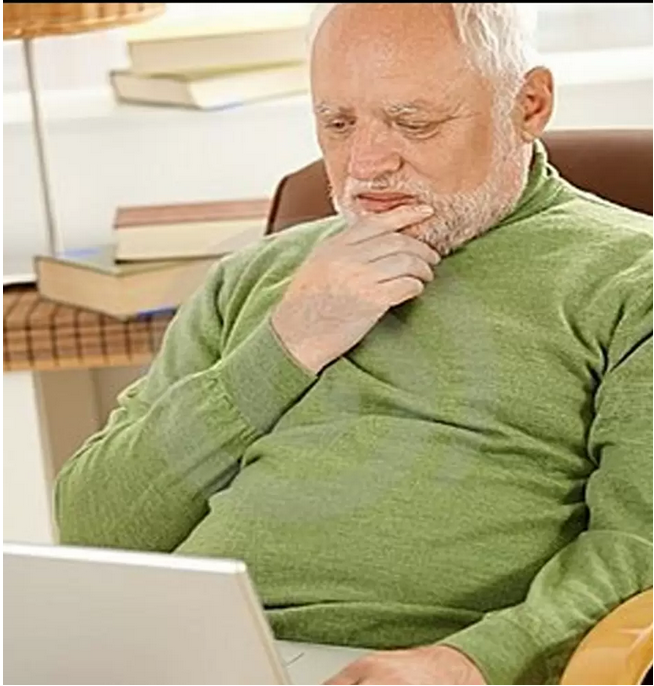
\includegraphics[width=1\textwidth]{figuras/haroldpensando.jpg}
             \end{center}
        \end{column}
    \end{columns}
\end{frame}

\begin{frame}{Usuários}
    \begin{columns}
        \begin{column}{0.65\textwidth}
            \begin{enumerate}[label=•]
                \item Pessoas que pretendem ter uma melhor gestão financeira
                \item Usuários de planilhas que desejam automatizar processos
                % \item Melhor controle e organização de gastos
            \end{enumerate}
        \end{column}
        
        \begin{column}{0.35\textwidth}
            \begin{center}
                
\includegraphics[width=1\textwidth]{figuras/haroldusuarios.png}
             \end{center}
        \end{column}
    \end{columns}
\end{frame}

\section{Problema 2:\newline Dificuldade ao contemplar curtas ou longas-metragens em grupo de modo que cada indivíduo possa fazê-lo diretamente de sua respectiva residência através da internet}

\begin{frame}{O que é o problema}
    \begin{columns}
        \begin{column}{0.65\textwidth}
            \begin{enumerate}[label=•]
                \item Assistir combinado sem um programa intermediador acaba resultando em perda de sincronia
                \item Pouca imersão
                \item Falta de interação entre usuários
            \end{enumerate}
            
            % \vspace{2mm}
            % Todos esses fatores requerem muita disciplina do usuário
        \end{column}
        \begin{column}{0.35\textwidth}
            \begin{center}
                
\includegraphics[width=1\textwidth]{figuras/harolddesgosto}
             \end{center}
        \end{column}
    \end{columns}
\end{frame}

\begin{frame}{O que é a solução}
    \begin{columns}
        \begin{column}{0.65\textwidth}
        \textbf{Simulador de cinema por realidade virtual (RV)}
            \begin{enumerate}[label=•]
                \item Altíssimo nível de imersão através do sistema de realidade virtual
                \item Qualidade \& Sincronia™
                \item Maior interação entre usuários
                \item Possibilidade de criar sessões com grande número de usuários
            \end{enumerate}
            
            \vspace{3mm}
            \textbf{\textcolor{red}{DD aprova!}}
        \end{column}
        \begin{column}{0.35\textwidth}
            \begin{center}
                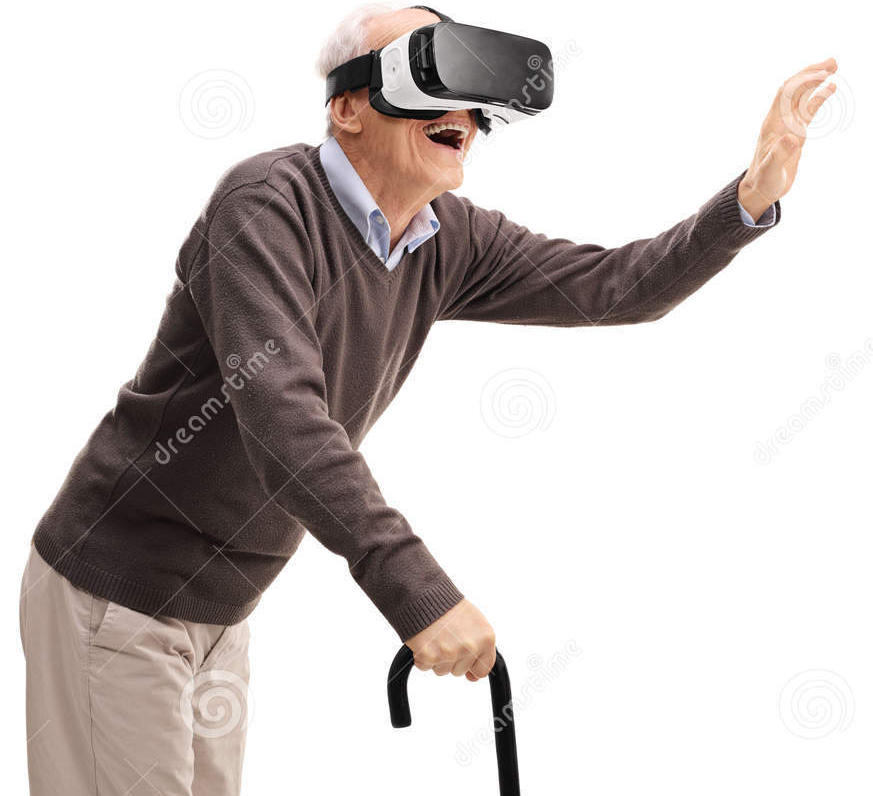
\includegraphics[width=1\textwidth]{figuras/ddaprova}
             \end{center}
        \end{column}
    \end{columns}
\end{frame}

\begin{frame}{Funções principais}
    \begin{enumerate}[label=•]
        \item Criação de salas (sessões)
        \item Escolha de arquivos disponíveis na máquina do host
        \item Escolha de modelos diferentes de salas
        \item Chat de voz e por teclado
        \item Lista de amigos dentro do jogo para fácil conexão
        \item Criação de grupos entre amigos para não atrapalhar a experiência de outros usuários
    \end{enumerate}
\end{frame}


\begin{frame}{Pontos fracos da solução}
    \begin{columns}
        \begin{column}{0.65\textwidth}
            \begin{enumerate}[label=•]
        		\item Requer equipamento de realidade virtual e um computador robusto
        		\item Considerável custo para desenvolvimento
        % 		\item Impossibilidade de trocar afetos
            \end{enumerate}
        \end{column}
        
        \begin{column}{0.35\textwidth}
            \begin{center}
                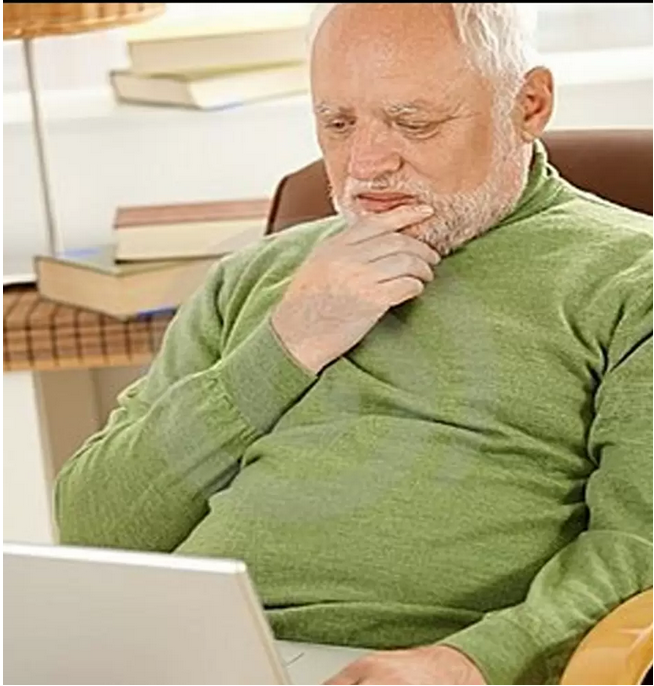
\includegraphics[width=1\textwidth]{figuras/haroldpensando.jpg}
             \end{center}
        \end{column}
    \end{columns}
\end{frame}

\begin{frame}{Usuários}
    \begin{columns}
        \begin{column}{0.65\textwidth}
            \begin{enumerate}[label=•]
        		\item Pessoas interessadas em RV em geral
        		\item Pessoas que querem assistir filmes com imersão em casa
        		\item Amigos que moram longe e desejam simular uma sessão de cinema
                \item Webnamorados
            \end{enumerate}
        \end{column}
        
        \begin{column}{0.35\textwidth}
            \begin{center}
                
\includegraphics[width=1\textwidth]{figuras/haroldusuarios.png}
             \end{center}
        \end{column}
    \end{columns}
\end{frame}

\begin{frame}[standout]{REFLITÃO}
    \begin{figure}
        
\includegraphics[scale=0.35]{figuras/reflitao.png}
    \end{figure}
\end{frame}

% \begin{frame}[fragile]{Introdução}

%     • Objetivo: ter precisão de pensamento e linguagem para obter a certeza matemática a respeito de um determinado problema.

%     • Métodos de Prova:
%     \vspace{-2mm}
%     \begin{itemize}
%         \item[--] Prova direta
%         \item[--] Contra-exemplo
%         \item[--] Divisão por casos
%         \item[--] Prova por contradição
%         \item[--] Prova por contraposição
%     \end{itemize}
% \end{frame}

    
% \begin{frame}{Prova direta: Definições}
%     \cite{Knuth92}, \citet{ConcreteMath}, \citeauthor{Er01}.
% \end{frame}

% \begin{frame}[allowframebreaks]{References}

%   \bibliography{demo}
  
  %\bibliographystyle{abbrv}

% \end{frame}

\end{document}
